\documentclass[a4paper,11pt]{article}
\usepackage[margin=2.5cm]{geometry} % Make more reasonable margins in document
\usepackage[parfill]{parskip}  % Remove LaTeX indents, and add interparagraph space
\usepackage[utf8]{inputenc}
\usepackage[english]{babel}

\usepackage{enumitem} % Enumerations met letters in de plaats van cijfers

%%%%%%%%%%%%
%%% MATH %%%
%%%%%%%%%%%%
\usepackage{mathtools}
\usepackage{amssymb}
\usepackage[output-decimal-marker={,}]{siunitx}
\usepackage{amsmath}
\newcommand\Log[1]{ \mathop{{}^{#1}\mathrm{log}} }
\DeclarePairedDelimiterX{\norm}[1]{\lVert}{\rVert}{#1}

% https://tex.stackexchange.com/questions/94032/fancy-tables-in-latex
\usepackage[table]{xcolor}
\usepackage{booktabs}

\usepackage[utf8]{inputenc}
\usepackage{pdfpages}

%Visuals
\usepackage{graphicx}
\usepackage{subcaption}
\usepackage[colorlinks,allcolors=violet]{hyperref}
\usepackage{url}
\usepackage[T1]{fontenc}
\usepackage{lmodern} 
\usepackage{algorithm}
\floatname{algorithm}{Algoritme}
\usepackage{algorithmic}
\usepackage{courier}
\usepackage{wrapfig}
\usepackage[export]{adjustbox}
\usepackage{wasysym}

%Figures
\usepackage{pgfplots}
\pgfplotsset{compat=newest}
%% the following commands are needed for some matlab2tikz features
\usetikzlibrary{plotmarks}
\usetikzlibrary{arrows.meta}
\usepgfplotslibrary{patchplots}
\usepackage{grffile}
\usepackage{caption}
\usepackage{float}
\usepackage{cleveref}
\usepackage{multirow}
\usepackage{titlesec}
\usepackage{listings}

\usepackage{multicol}
\usepackage{tikz}
\lstset{
	language=Matlab,
	%    basicstyle={\ttfamily \small},
	basicstyle={\ttfamily \small},
	%    keywordstyle=\underline,
	numberstyle={\footnotesize},
	%    morekeywords={ones,mod,isprime,inline,unique,factor,@},
	%    flexiblecolumns=false,
	%    emph={gamma,beta},
	%    emphstyle=,
	columns=fullflexible,
	%    columns=flexible,
	%    commentstyle={\slshape},
	%    commentstyle={\normalfont},
	commentstyle={\ttfamily},
	stringstyle={\ttfamily \bfseries},
	showstringspaces=false,
	%    indent=1em,
	%    xleftmargin=0.5em,
	breaklines=false,
	%    frame={l},
	captionpos={t},
	upquote=true, % such that we can copy-paste the code...
	%    mathescape=true,
	%    frame=single,     % boxed in a single line
	%    frame=L,          % double line on the left
	%    frame=l,          % single line on the left
}

\newcommand*\circled[1]{\tikz[baseline=(char.base)]{
            \node[shape=circle,draw,inner sep=0.1pt] (char) {#1};}}
\newcommand{\note}[1]{{\colorbox{yellow!40!white}{#1}}}
\titleformat{\section}
{\normalfont\Large\bfseries}{\boxed{\text{Assignment \thesection}}}{1em}{}

\setlength{\pdfpageheight}{11in}


\title{Nonlinear Systems \\[1ex]
    \Large \textsc{Assignments}}
\author{Elias Wils}
\date{\today}

\begin{document}

\maketitle
\newpage
\tableofcontents

\newpage
\section{Stability of equilibrium points and bifurcations}    
\subsection{A simple population model}
\paragraph{Question 1}\: The position and number of equilibrium points depends on the value of $\alpha$ and $\beta$.
In \Cref{tbeq1} the different possible cases are listed together with information about the equilibrium points.
When looking at the graph of $\dot{N}$ against $N$, a negative parabola can be observed, intersecting the $N$-axis in two points.
When solving the quadratic equation for $\dot{N}=0$ with $\alpha$ and $\beta$ as unknown parameters, expressions shown in (1) and \eqref{eqN2} for
the equilibrium points ensue.
\begin{align}
	N_1 &= 0\\
	N_2 &= \frac{K(\alpha-\beta)}{\alpha}
	\label{eqN2}
\end{align}
\begin{table}[H]
	\centering
	\begin{tabular}{|c|c|c|}
	\hline
	$\alpha<\beta$ & $\alpha>\beta$ & $\alpha=\beta$\\
	\hline
	$N_1$ is stable (\CIRCLE) & $N_1$ is unstable (\Circle) & $N_1=N_2$\\
	$N_2$ is unstable (\Circle) & $N_2$ is stable (\CIRCLE) & half stable equilibrium point (\RIGHTcircle)\\
	\hline
	\end{tabular}
	\captionsetup{width=0.9\textwidth}
	\caption{Summary of the characteristics of the equilibrium points for different cases of $\alpha$ and $\beta$. }
	\label{tbeq1}
\end{table}
The type of bifurcation that occurs here is called transcritical. A qualitative representation of this bifurcation can be seen in 
\Cref{fig:trbif}, with the different cases in the same order as in \Cref{tbeq1}. Here the x-axis represents $N$, and the 
y-axis represents $\dot{N}$
\begin{figure}[H]
	\centering
	\makebox[\textwidth][c]{
	\begin{subfigure}{0.45\linewidth}
		\centering
		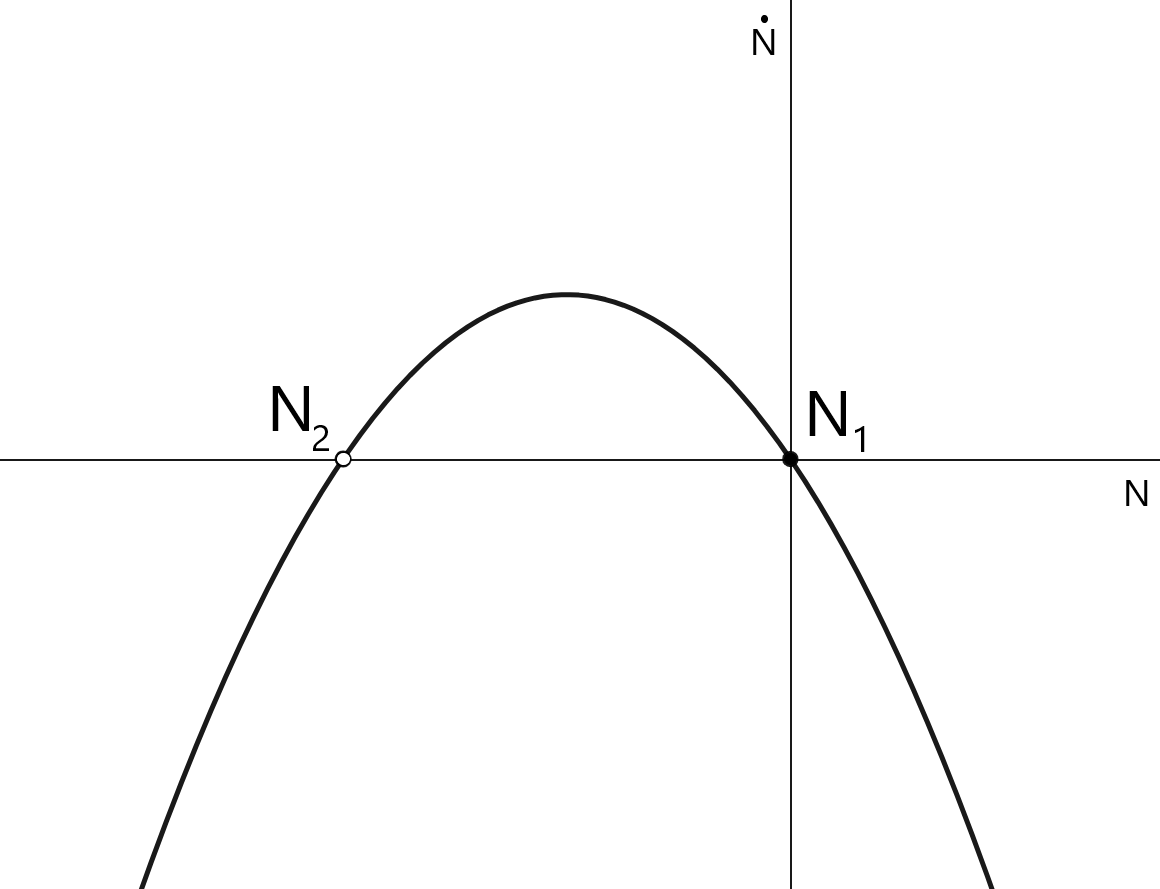
\includegraphics[width=\textwidth]{altb.png}
		\caption{$\alpha<\beta$}
	\end{subfigure}\hfill
	\begin{subfigure}{0.45\linewidth}
		\centering
		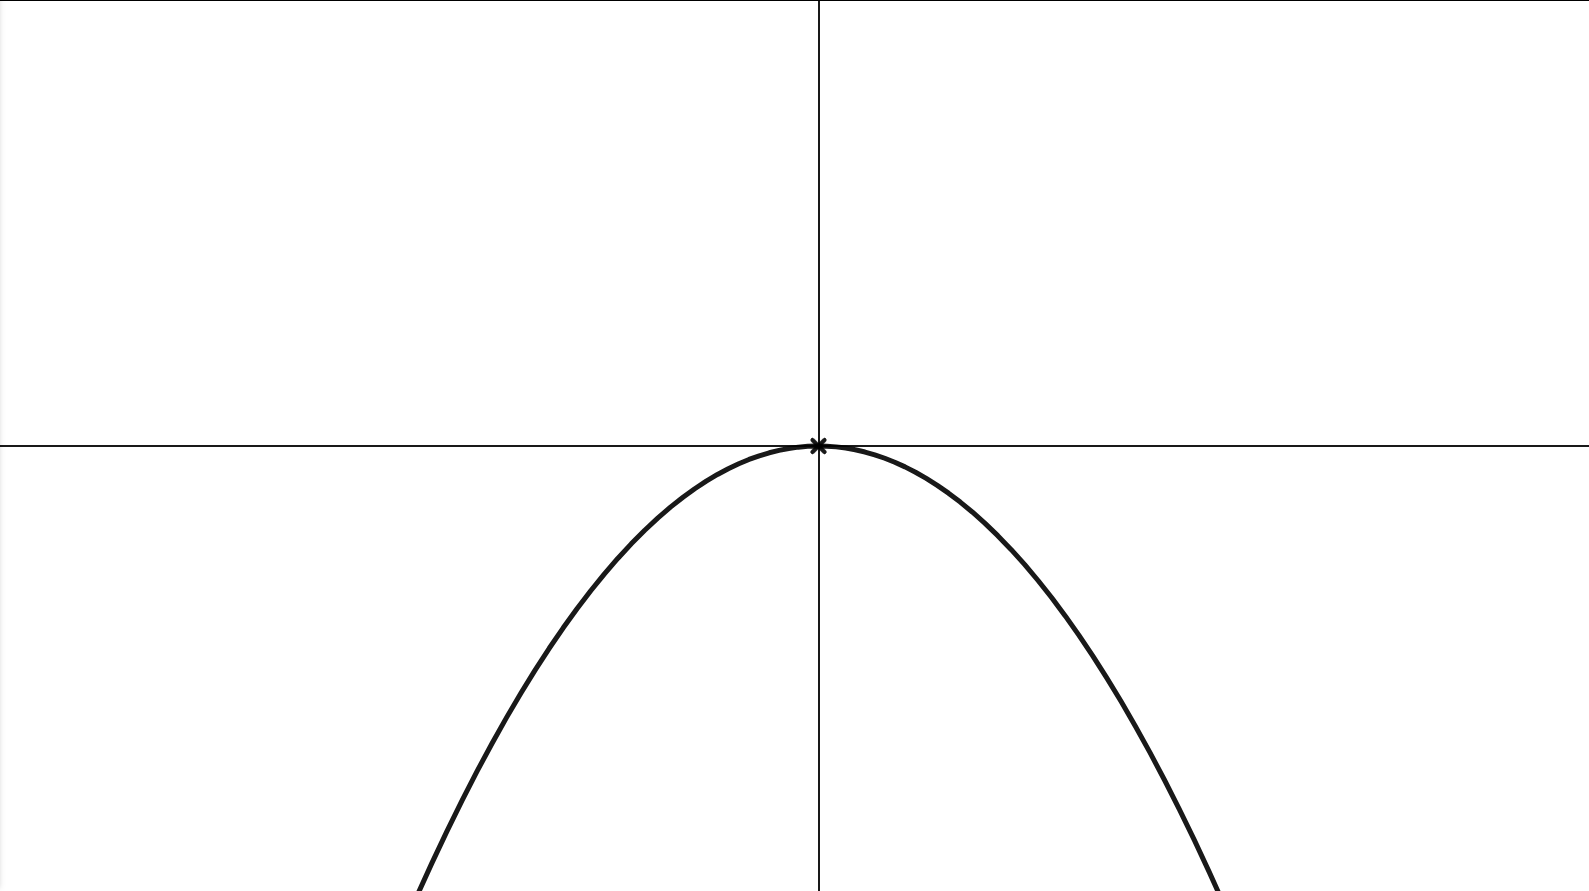
\includegraphics[width=\textwidth]{aisb.png}
		\caption{$\alpha=\beta$}
	\end{subfigure}
	\begin{subfigure}{0.45\linewidth}
		\centering
		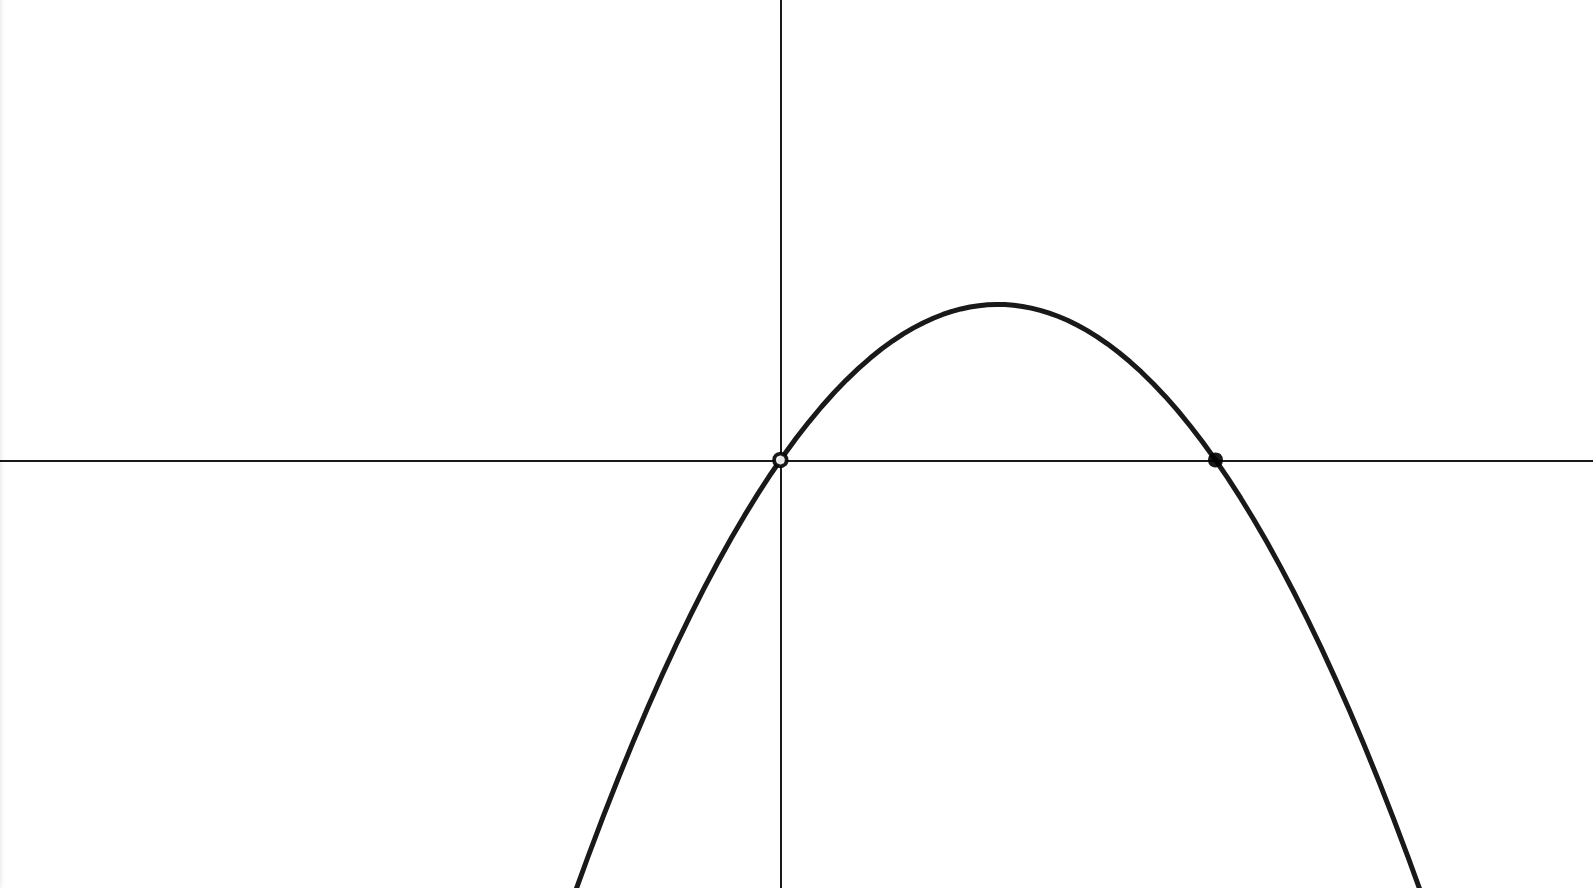
\includegraphics[width=\textwidth]{agtb.png}
		\caption{$\alpha>\beta$}
	\end{subfigure}
	}
	\caption{Qualitative plot of $\dot{N}$ against N for the different cases for $\alpha$ and $\beta$.}
	\label{fig:trbif}
\end{figure}
\paragraph{Question 2}\: For the practical example described here, the solution for $t\rightarrow\inf$ will converge to one 
of the equilibrium points. As $\alpha>\beta$, the second case in \Cref{tbeq1} is applicable. The only stable equilibrium point
is $N_2=\frac{K(\alpha-\beta)}{\alpha}=10\:470\:086$. Thus, with the parameters declared in the assignment text,
the number of inhabitants will converge towards the stable equilibrium $N_2$, which is $10\:470\:086$ here, as 
$t\rightarrow\infty$.\\

\subsection{Gene control model}
\paragraph{Question 1}\: When taking the repression rate $r=0$, only one fixed point is visible. 
The system equations become:
\begin{equation*}
	\begin{cases}
		 \dot{x}=\frac{\alpha_1}{2}-x\\
		 \dot{y}=\frac{\alpha_2}{2}-y
	\end{cases}
\end{equation*}
The only fixed point is $\left(\frac{\alpha_1}{2}, \frac{\alpha_2}{2}\right)$. We can classify fixed points
of a 2-dimensional system by analyzing the system matrix. As this system is nonlinear The Jacobian is taken 
as an approximation of this system matrix. Then the system becomes linear and an appropriate stability analysis
can be done. Below the computations are first done for the general case, whereafter $r=0$ is filled in.
The Jacobian of this nonlinear system becomes:
\begin{equation*}
	J=
	\begin{bmatrix}
		-1 & -\frac{\alpha_1ry^{r-1}}{(y^r+1)^2}\\
		-\frac{\alpha_2rx^{r-1}}{(x^r+1)^2} & -1
	\end{bmatrix}=
	\begin{bmatrix}
		-1 & 0\\
		0 & -1
	\end{bmatrix}
\end{equation*}
The trace $\tau$ of this matrix is $-2$ and the determinant $\Delta$ is:
\begin{equation*}
	\Delta=1-\frac{\alpha_1\alpha_2r^2x^{r-1}y^{r-1}}{(x^r+1)^2(y^r+1)^2}=1
\end{equation*}
In the Strogatz book there is summarized how fixed points can be classified through
$\tau$ and $\Delta$. Here $\tau<0$ and $\Delta>0$, and $\tau^2-4\Delta=0$. This means that this fixed
point is a \textbf{degenerate node}. It lies on the border between nodes and spirals, and it means that the 
eigenspace corresponding to the only eigenvalue is one-dimensional.
\paragraph{Question 2}\: $\alpha_1=\alpha_2=2$ and $r>0$.
\vspace{-5	mm}
\paragraph{i.}\: An obvious fixed point here is $(1, 1)$, and this is verified by \texttt{PPLANE},
as seen in \Cref{fig:pp1}, where a value of $r=1$ is used. 
\vspace{-5mm}
\paragraph{ii.}\: When studying the stability, there can again be made use of the Jacobian derived earlier and
fill in the given values for the parameters and $(x,y)=(1,1)$.
\begin{equation*}
	J=
	\begin{bmatrix}
		-1 & -\frac{\alpha_1ry^{r-1}}{(y^r+1)^2}\\
		-\frac{\alpha_2rx^{r-1}}{(x^r+1)^2} & -1
	\end{bmatrix}=
	\begin{bmatrix}
		-1 & -\frac{r}{2}\\
		-\frac{r}{2} & -1
	\end{bmatrix}
\end{equation*}
The expression for the determinant then becomes:
\begin{equation*}
	\Delta=1-\frac{\alpha_1\alpha_2r^2x^{r-1}y^{r-1}}{(x^r+1)^2(y^r+1)^2}=1-\frac{r^2}{4}
\end{equation*}
The trace $\tau$ stays -2. For $0< r< 2$, $\tau<0$ and $\Delta>0$ just as in Question 1.
However, now $\tau^2-4\Delta>0$, so for this range for $r$ $(1,1)$ is a stable node.\\ The special case
where $r=0$ is worked out in Question 1, then $(1,1)$ is a degenerate node. \\
Then also $r=2$ deviates from the rest. The determinant $\Delta$ then becomes zero, which means that one
of the eigenvalues is zero as the Jacobian becomes a matrix of just $-1$s. When $r$ exceeds 2, the determinant
$\Delta$ becomes negative, which means a saddle node is established.\\
These findings are summarized in \Cref{tbeq2}.
\begin{table}[H]
	\centering
	\begin{tabular}{|c|c|c|c|}
	\hline
	$r=0$ & $0<r<2$ & $r=2$ & $r>2$\\
	\hline
	$\tau=-2<0$ & $\tau=-2<0$ & $\tau=-2<0$ & $\tau=-2<0$\\
	$\Delta=1>0$ & $\Delta\in(0,1)>0$ & $\Delta=0$ & $\Delta<0$\\
	$\tau^2-4\Delta=0$ & $\tau^2-4\Delta\in(0,4)>0$ & $\tau^2-4\Delta=4>0$ & $/$\\
	degenerate node & stable node & stable line of nodes & saddle node\\
	\hline
	\end{tabular}
	\captionsetup{width=0.9\textwidth}
	\caption{Summary of the characteristics of the fixed point $(1,1)$ for $0\leq r\leq2$.}
	\label{tbeq2}
\end{table}
\vspace{-5mm}
The phase portraits for these cases are shown in \Cref{fig:pp1}, as requested in \textbf{iv}.
\vspace{-3mm}
\paragraph{iii.}\: There can be noticed that a bifurcation occurs when $r$ crosses the value 2. This bifurcation is a 
supercritical pitchfork bifurcation, because when $r>2$, a pair of stable equilibrium points appear symmetrically w.r.t. the fixed point $(1,1)$.
This fixed point $(1,1)$ is stable when $0<r<2$ and becomes unstable when $r>2$ as it becomes a saddle node.
These types of bifurcations occur in systems where there is some sort of symmetry present, as is the case here.
The two system equations are exactly the same, apart from the fact that $x$ and $y$ are interchanged. This also causes the 
Jacobian to be almost symmetrical, apart from the interchanged $x$ and $y$ again.\\
This is also seen when computing the phase plane numerically with \texttt{PPLANE}. Once $r$ exceeds 2, 
two more fixed points arise symmetrical w.r.t. the original fixed point $(1,1)$.

\paragraph{iv.}\: The phase portraits for the different cases of $r$ listed in \Cref{tbeq2} are shown in \Cref{fig:pp1}.
\begin{figure}[H]
	\centering
	\makebox[\textwidth][c]{
	\begin{subfigure}[b]{0.5\textwidth}
		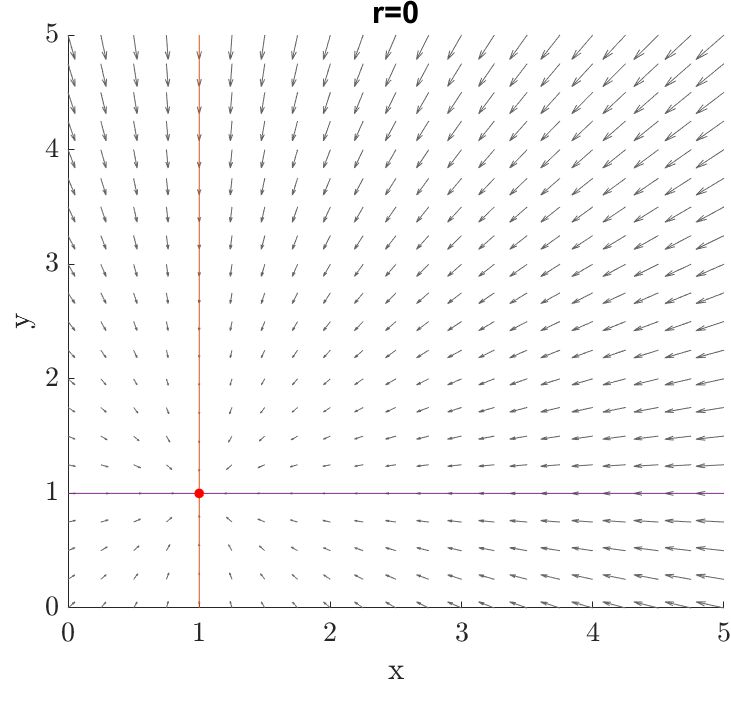
\includegraphics[width=\textwidth]{r0.png}
		\caption{Phase portrait for $r=0$.}
		\label{fig:r0} 
	\end{subfigure}

	\begin{subfigure}[b]{0.5\textwidth}
		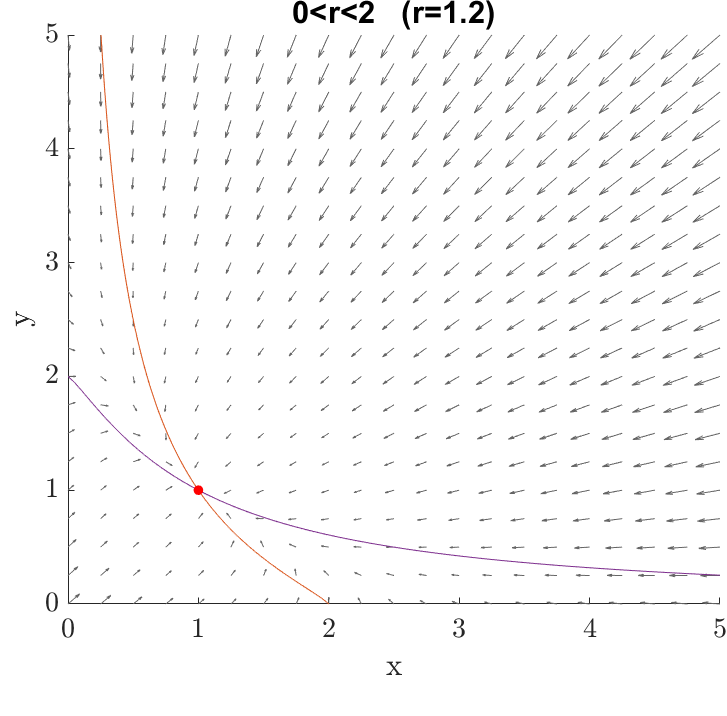
\includegraphics[width=\textwidth]{0r2.png}
		\caption{Phase portrait for $r=1.2$.}
		\label{fig:0r2}
	\end{subfigure}
	}
	\makebox[\textwidth][c]{
	\begin{subfigure}[b]{0.5\textwidth}
		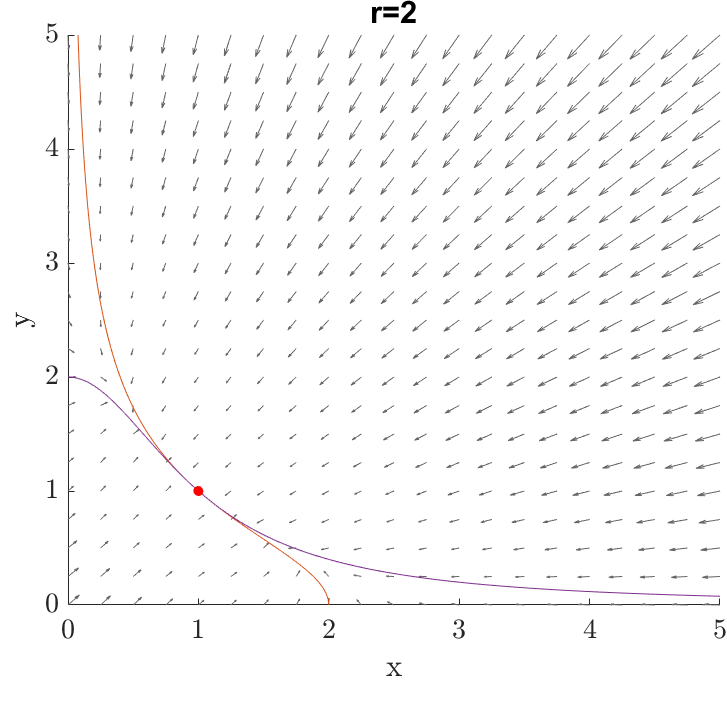
\includegraphics[width=\textwidth]{r2}
		\caption{Phase portrait for $r=2$.}
		\label{fig:r2} 
		\end{subfigure}
		
		\begin{subfigure}[b]{0.5\textwidth}
		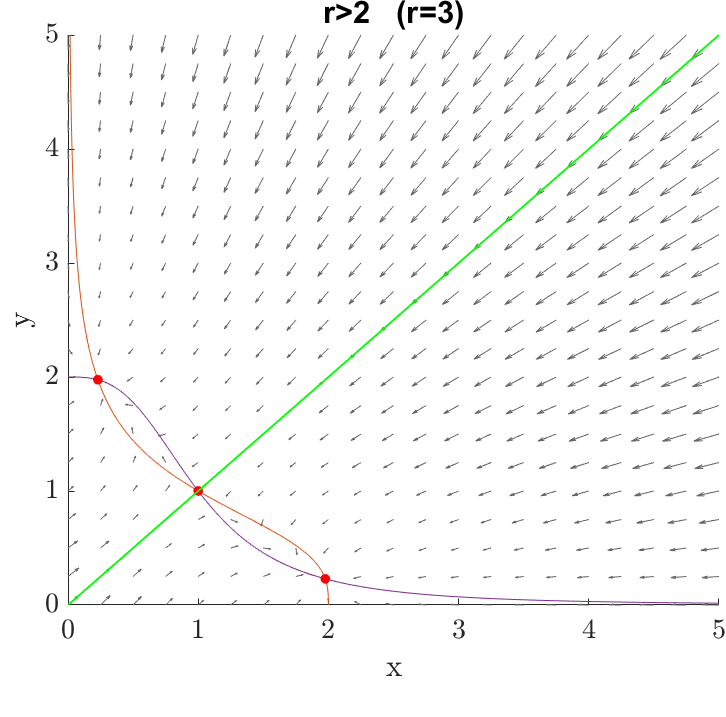
\includegraphics[width=\textwidth]{rgt2.png}
		\caption{Phase portrait for $r=3$.}
		\label{fig:rgt2}
		\end{subfigure}
	}
	\label{fig:pp1}
	\vspace{-3mm}
	\caption{Phase portraits of the given system for the qualitatively different phase portraits when varying $r$.}
\end{figure}
The bifurcation that occurs here is a supercritical pitchfork bifurcation, and a qualitative sketch of the bifurcation diagram of
either $x$ or $y$ is shown in \Cref{fig:bif}.
\begin{figure}[H]
	\centering
	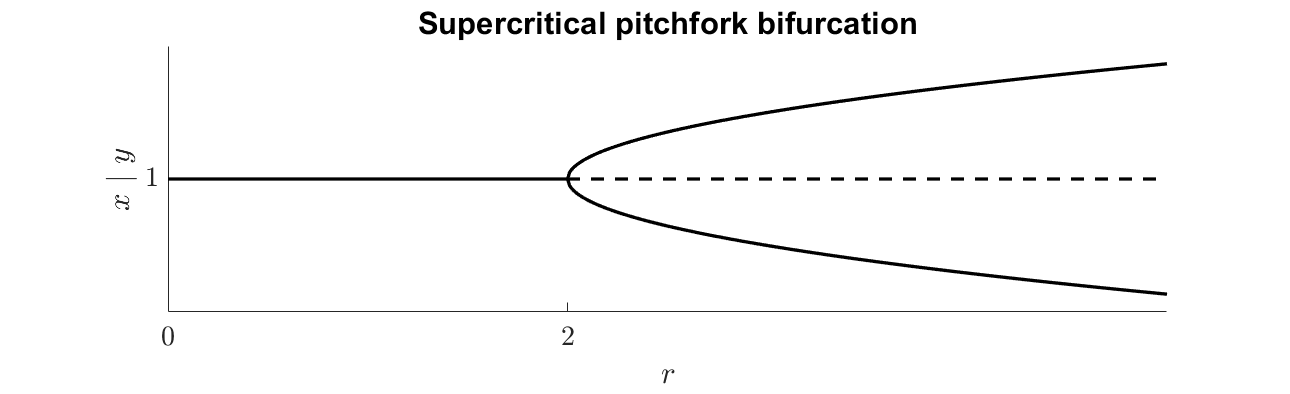
\includegraphics[width=1.1\textwidth]{suppit.png}
	\caption{Qualitative bifurcation diagram of the supercritical pitchfork bifurcation.}
	\label{fig:bif} 
\end{figure}

\newpage
\section{Imperfect bifurcations}
\subsection{Gene control revisited}
The accurate bifurcation diagram using \texttt{COCO} can be found in \Cref{fig:bif1}. The diagram for both
$x$ and $y$ in function of $r$ is plotted, as the diagram 3-dimensional.
\begin{figure}[H]
	\centering
	\makebox[\textwidth][c]{
	\begin{subfigure}[b]{0.5\textwidth}
		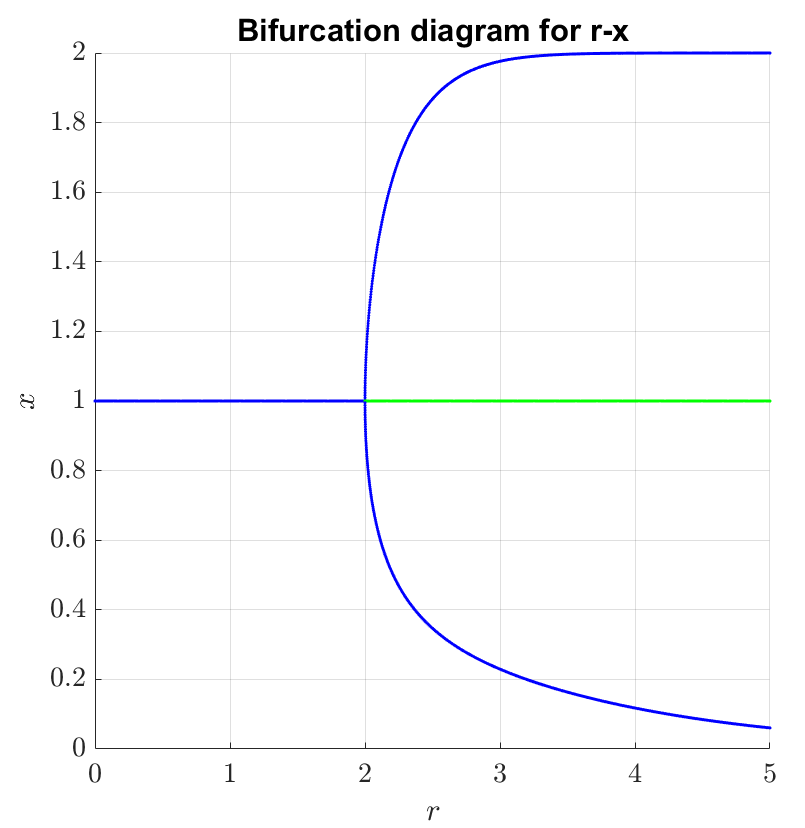
\includegraphics[width=\textwidth]{bif1x.png}
		\caption{Pitchfork for $r$ and $x$.}
		\label{fig:bif1x} 
	\end{subfigure}\hfill

	\begin{subfigure}[b]{0.503\textwidth}
		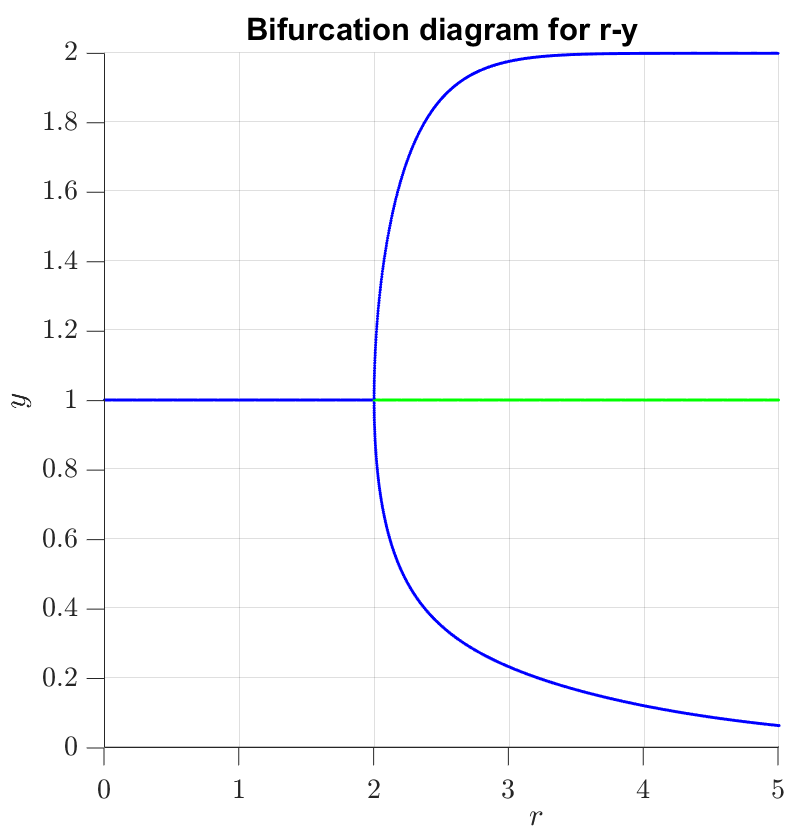
\includegraphics[width=\textwidth]{bif1y.png}
		\caption{Pitchfork for $r$ and $y$.}
		\label{fig:bif1y}
	\end{subfigure}
	}
	\label{fig:bif1}
	\caption{Bifurcation diagram of the supercritical pitchfork bifurcation in both $x$ and $y$, obtained with \texttt{COCO}.}
\end{figure}
The blue line represents the stable equilibrium points, while the green line represents the 
saddle nodes that become present when $r>2$. The supercritical pitchfork bifurcation can be noticed very well.

\subsection{Imperfect bifurcations}
\paragraph{Question 1}\: The bifurcation diagram of the given equilibrium equation can be plotted for different values of $r$ 
in function of $h$ and $x$. When $-1\leq r\leq0$, the bifurcation diagram has no turning points present, and consists of one 
continuous curve of stable equilibrium points.\\
When $0<r\leq1$, two turning points arise in a symmetric fashion, together with a branch of unstable equilibrium points
in the middle. \\
The transition between those two cases arises when $r=0$. Then the point $(x,h)=(0,0)$ is a non-generic turning point (or degenerate fold).
This non-generic turning point is indicated by a red dot in \Cref{fig:bifhxr0}.
The bifurcation diagrams of these cases are shown in \Cref{fig:bifhx}.

\begin{figure}[H]
	\centering
	\makebox[\textwidth][c]{
	\begin{subfigure}{0.43\linewidth}
		\centering
		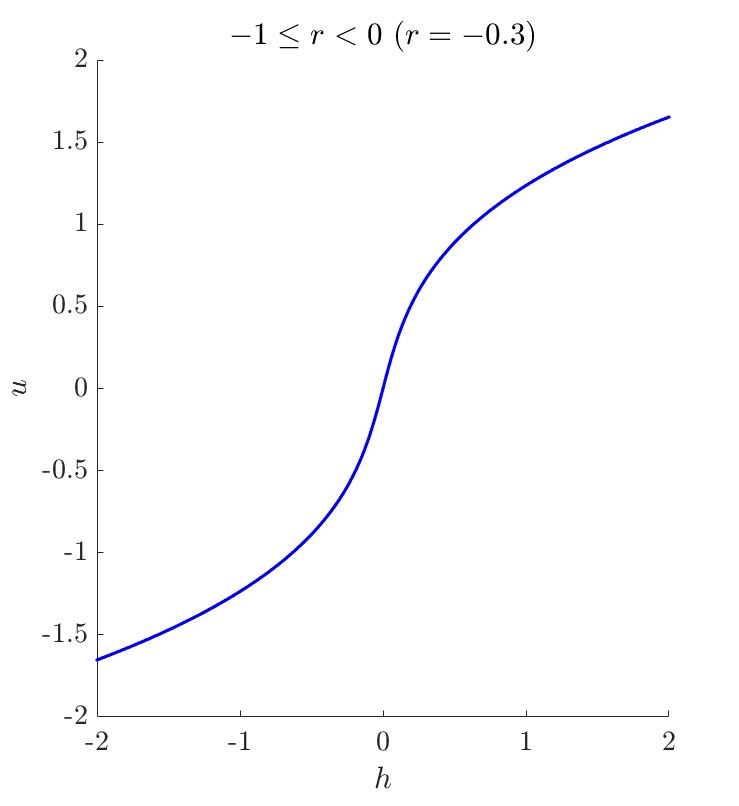
\includegraphics[width=\textwidth]{bifhxr-1.png}
		\caption{$r\in[-1,0)$, here $r=-0.3$}
	\end{subfigure}\hfill
	\begin{subfigure}{0.43\linewidth}
		\centering
		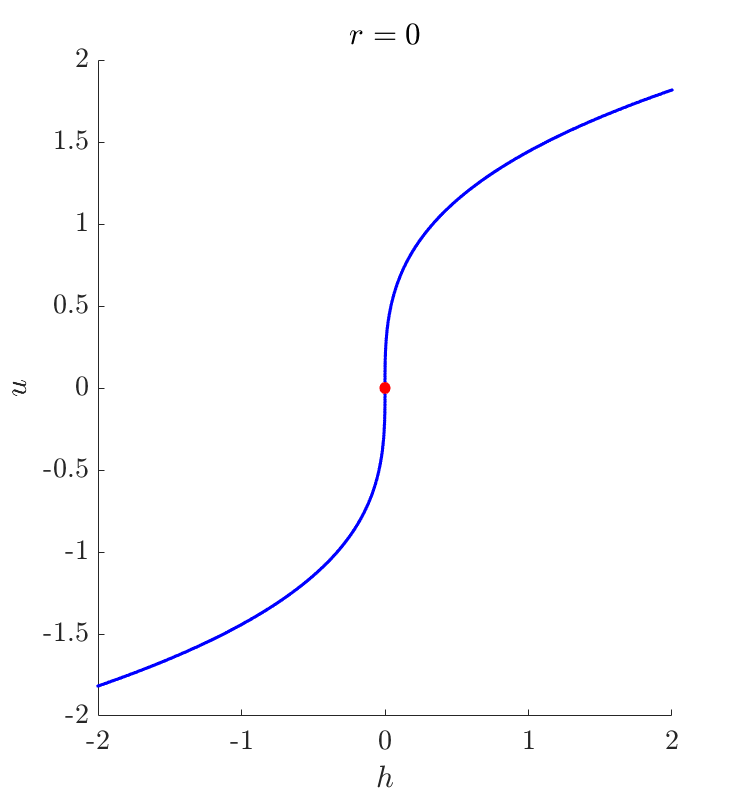
\includegraphics[width=\textwidth]{bifhxr0.png}
		\caption{$r=0$}
		\label{fig:bifhxr0}
	\end{subfigure}
	\begin{subfigure}{0.43\linewidth}
		\centering
		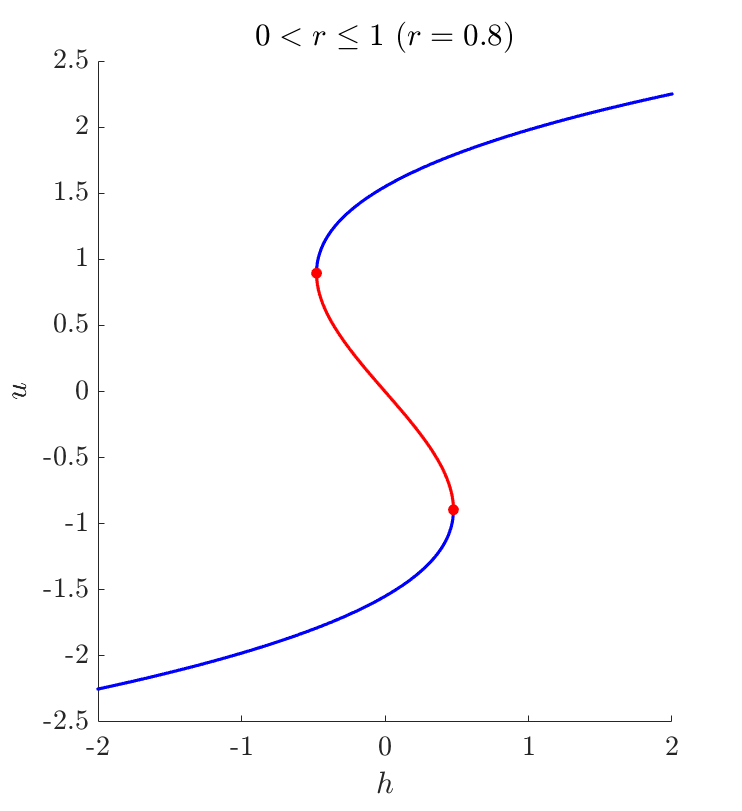
\includegraphics[width=\textwidth]{bifhxr1.png}
		\caption{$r\in(0,1]$, here $r=0.8$.}
	\end{subfigure}
	}
	\caption{Bifurcation diagrams in function of $h$ for different values of $r$.}
	\label{fig:bifhx}
	\vspace{-4mm}
\end{figure}

\paragraph{Question 2}\: Then also the bifurcation diagram can be plotted for different values of $h$ 
in function of $r$ and $x$. The diagram is plotted in \Cref{fig:bifrx} for three values of $h$: $-0.1$, 0 and 1.\\
When $h=0$, a regular supercritical pitchfork can be seen.\\ When h is decreased under zero, for example $-0.1$, 
The pitchfork is separated into two separate smooth curves, one with stable equilibrium points, and one with
a turning point.\\
When $h>0$, for example 0.1, the pitchfork decomposes again, but this time in the opposite direction.
Again \\
The parameter $h$ serves as an \textit{imperfection parameter}, as it removes the symmetry of the pitchfork bifurcation
as $h\neq0$.
This imperfection parameter $h$ can also be seen as a perturbation of a model. In real life problems 
the model that is constructed doesn't always correspond exactly to reality.
$h$ can be interpreted as an additive perturbation, thus there can be explained why fixed points arise
and disappear when a model is perturbed.

\begin{figure}[H]
	\centering
	\vspace{-1mm}
	\makebox[\textwidth][c]{
	\begin{subfigure}{0.43\linewidth}
		\centering
		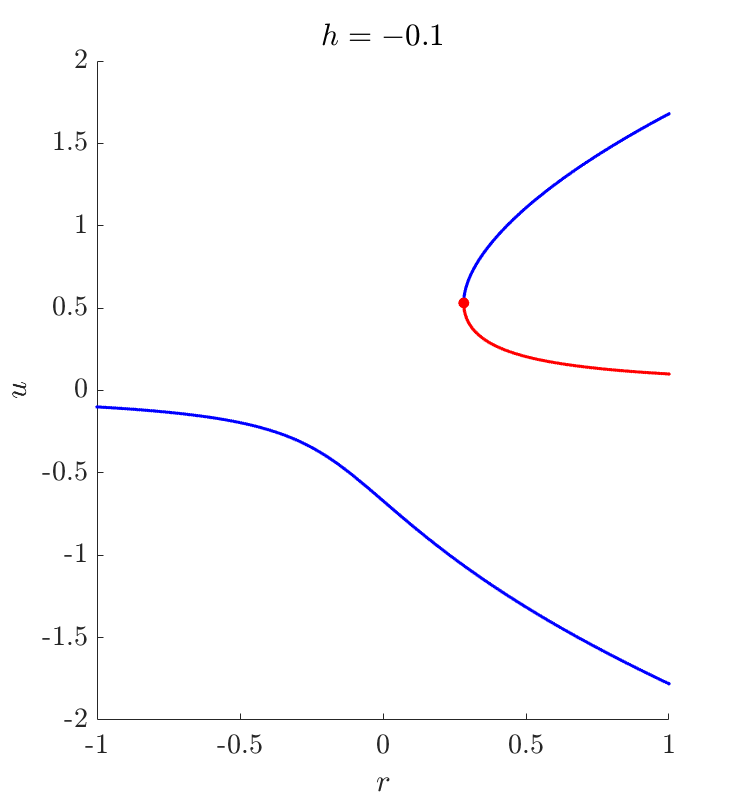
\includegraphics[width=\textwidth]{bifrxh-1.png}
		\caption{$h=-0.1$}
	\end{subfigure}\hfill
	\begin{subfigure}{0.43\linewidth}
		\centering
		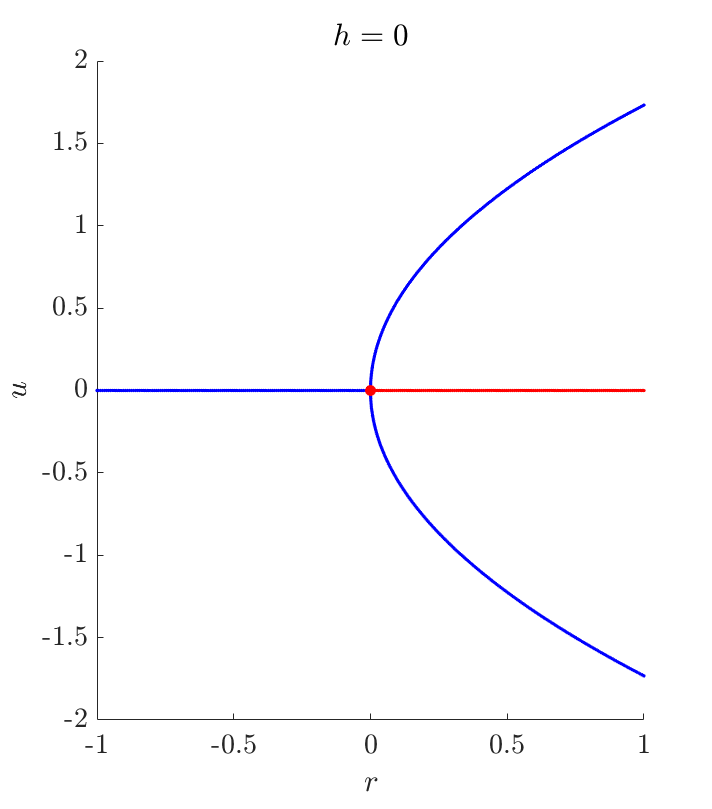
\includegraphics[width=\textwidth]{bifrxh0.png}
		\caption{$h=0$}
		\label{fig:bifrxh0}
	\end{subfigure}
	\begin{subfigure}{0.43\linewidth}
		\centering
		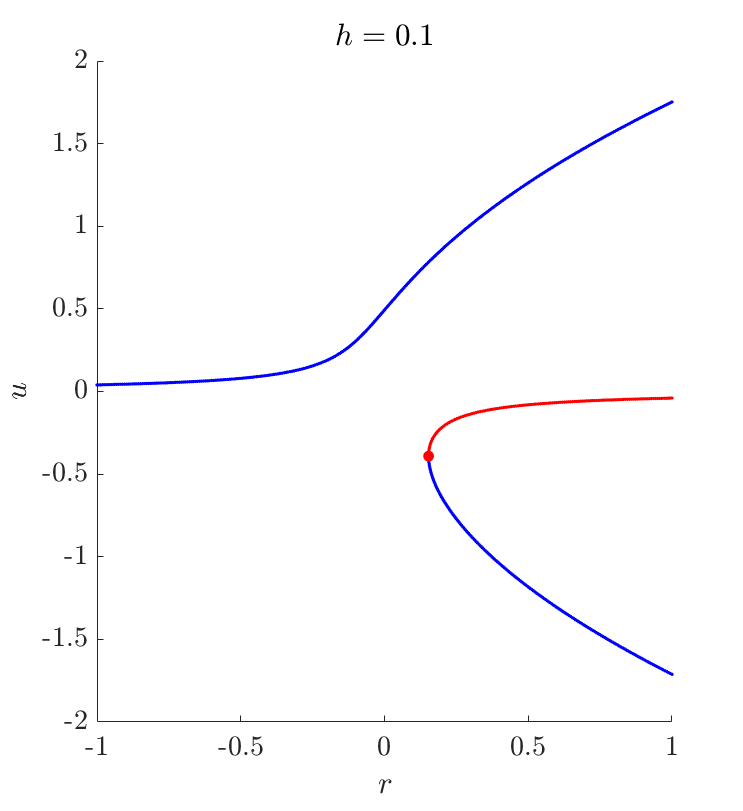
\includegraphics[width=\textwidth]{bifrxh1.png}
		\caption{$h=0.1$}
	\end{subfigure}
	}
	\caption{Bifurcation diagrams in function of $r$ for different values of $h$.}
	\label{fig:bifrx}
\end{figure}

\paragraph{Question 3}\: The fold curve was determined using \texttt{COCO}, and the result is shown in \Cref{fig:foldc}.
The projections on the $(u,r)$, $(u,h)$ and $(r,h)$ plane is plotted.
\begin{figure}[H]
	\centering
	\makebox[\textwidth][c]{
	\begin{subfigure}{0.43\linewidth}
		\centering
		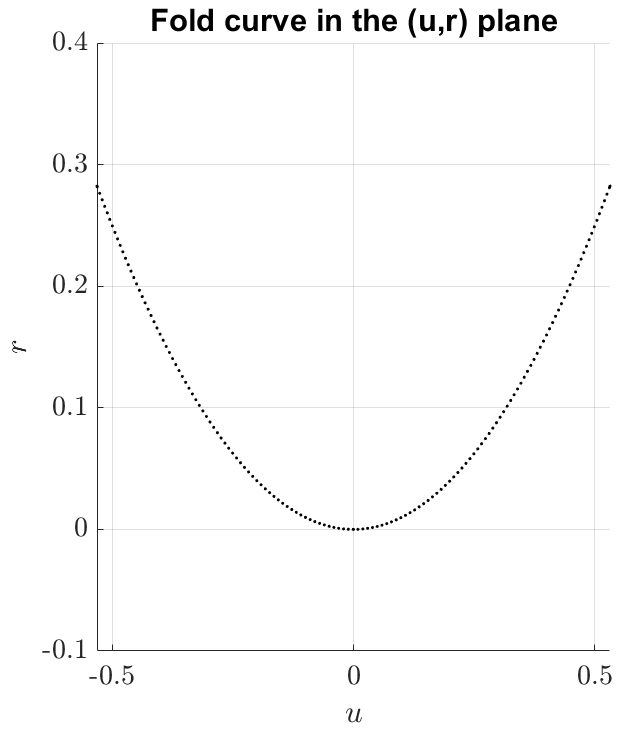
\includegraphics[width=\textwidth]{foldur.png}
		\caption{$(u,r)$ plane}
	\end{subfigure}\hfill
	\begin{subfigure}{0.43\linewidth}
		\centering
		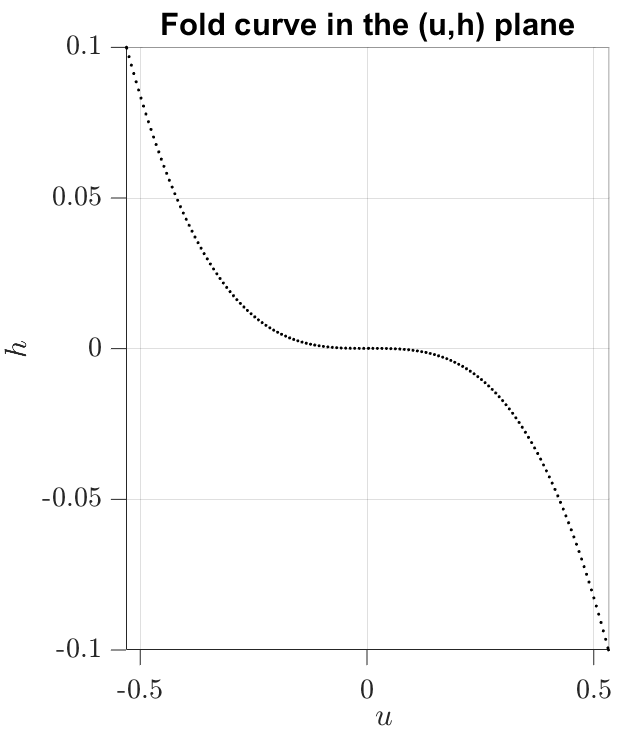
\includegraphics[width=\textwidth]{folduh.png}
		\caption{$(u,h)$ plane}
	\end{subfigure}
	\begin{subfigure}{0.43\linewidth}
		\centering
		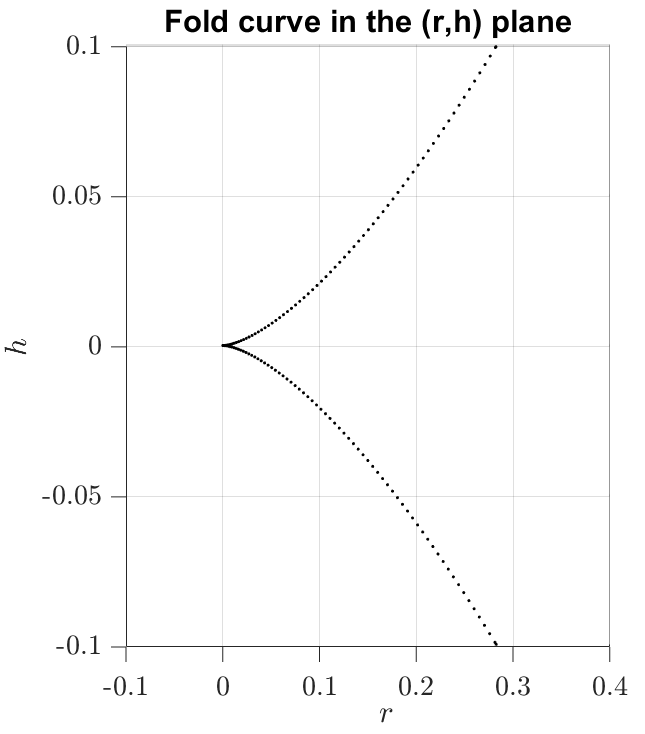
\includegraphics[width=\textwidth]{foldrh.png}
		\caption{$(r,h)$ plane}
		\label{fig:foldcrh}
	\end{subfigure}
	}
	\caption{Fold curve projected on the 2-dimensional $(u,r)$, $(u,h)$ and $(r,h)$ planes.}
	\label{fig:foldc}
\end{figure}
These three curves are the projections of the cusp catastrophe surface. When looking at the $(r,h)$ projection,
there can be noticed that when the curve is crossed, a \textit{catastrophe} occurs and the behaviour of the system
changes abruptly.\\
The correlation of the $(r,h)$ mapping (\Cref{fig:foldcrh}) with the bifurcation plots (\Cref{fig:bifhx} and \Cref{fig:bifrx})
is clearly visible. The point $(r,h)=(0,0)$ can be seen as a transition point, and it is also the starting point
of the fold curve in \Cref{fig:foldcrh}. In this point the system transitions from having one turning point, to having
three. The symmetry of this fold curve can also be seen through the plot at Question 1 (\Cref{fig:bifhx}), where 
two additional turning points arise when $h>0$ and drift away from each other in symmetrical fashion. When studying the evolution
of these fixed points and mapping it to the $(r,h)$ plane, the plot from \Cref{fig:foldcrh} can be constructed.\\
Also the other two mappings to the $(u,r)$ and $(u,h)$ plane can be constructed from looking at the evolution 
of the turning points in the plots from Question 1 and 2 (\Cref{fig:bifhx} and \Cref{fig:bifrx})

\paragraph{Question 4}\: For this question the influence of four continuation parameters within \texttt{COCO} was studied for 
a point very close to the cusp point. Namely the the bifurcation diagram in function of $r$ is asked for small 
negative values of $h$, so right at the point where the pitchfork breaks into two branches.
The bifurcation diagrams are depicted below in \Cref{fig:bifh}.
\begin{figure}[H]
	\centering
	\makebox[\textwidth][c]{
	\begin{subfigure}[b]{0.5\textwidth}
		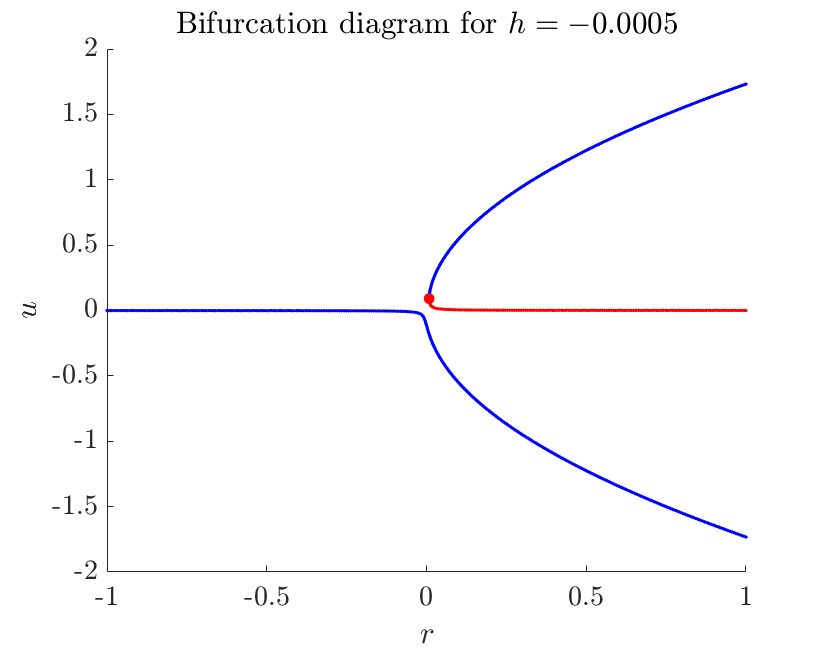
\includegraphics[width=\textwidth]{h5.png}
		\caption{\texttt{h\_max=0.05}}
	\end{subfigure}\hfill

	\begin{subfigure}[b]{0.5\textwidth}
		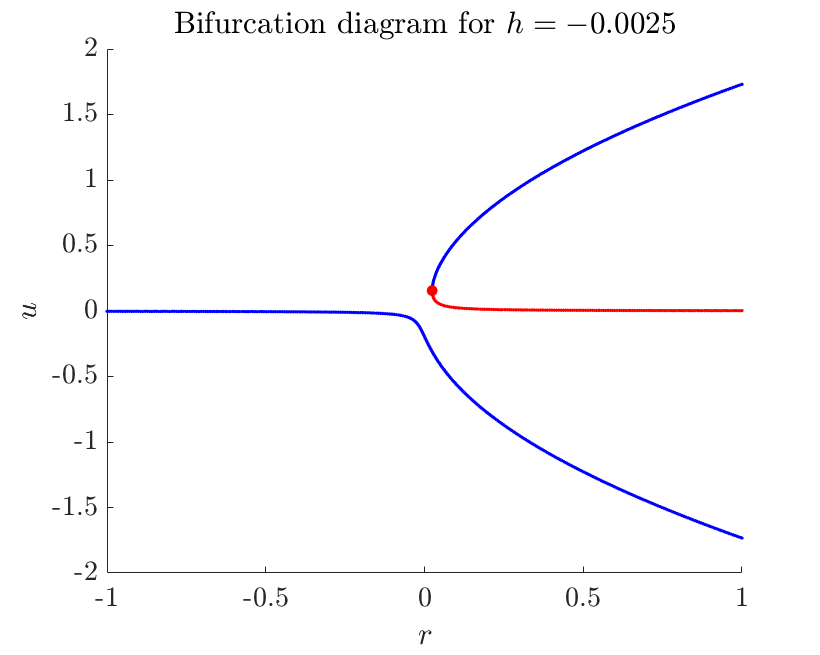
\includegraphics[width=\textwidth]{h25.png}
		\caption{\texttt{h\_max=0.05}}
	\end{subfigure}
	}
	\caption{Bifurcation diagrams in function of $r$ for $h=-0.0005$ and $h=-0.0025$, obtained with \texttt{COCO}.}
	\label{fig:bifh}
\end{figure}
These parameters are listed below, together with a short explanation and their influence on the result. Then also
a few plots are shown, which demonstrate the effects of these parameters when they are not set properly.\\
\begin{itemize}
	\item \texttt{h\_min}\: This is the minimum step size (incrementation of the parameter) for the continuation, in the course
	slides denoted as $\Delta\lambda$. This parameter allows to set a lower bound on this step size, so not more points are computed
	than necessary. \\When this bound is too large, an unwanted branch switch may occur. This is illustrated in \Cref{fig:bs}.
	For small values of $h$, this has a higher chance of happening, so the step size has to be small enough.
	\item \texttt{h\_max}\: This is the maximum step size $\Delta\lambda$. \\This parameter thus functions as an upper bound, and also
	needs to be small enough, otherwise the unwanted branch switch (\Cref{fig:bs}) can occur. For small $h$ it needs to be chosen small
	enough as well, but has to be larger than \texttt{h\_min} of course.
	\item \texttt{cont - ItMX}\: This parameter determines the maximum number of iterations during continuation. In other words,
	this parameter determines how many steps on a branch are taken at maximum. \\When a small step size is chosen, this parameter
	needs to be large enough, otherwise the branch may not be fully computed in the desired interval. In \Cref{fig:steps} is shown
	what happens when the parameter is too small.
	\item \texttt{corr - ItMX}\: This also functions as an upper bound on the number of iterations, but this time during the Newton
	correction of the gradient when a step is taken. If this parameter is chosen too small, the solution will be computed very inaccurately and will
	mostly look very different from the real solution.
	Luckily Newton doesn't need many iterations in our case (2-3), so a value 10 is more than enough. In general there probably won't be needed
	a lot of iterations because of the quadratic convergence of the Newton iteration.
\end{itemize}
\begin{figure}[H]
	\centering
	\makebox[\textwidth][c]{
	\begin{subfigure}[b]{0.5\textwidth}
		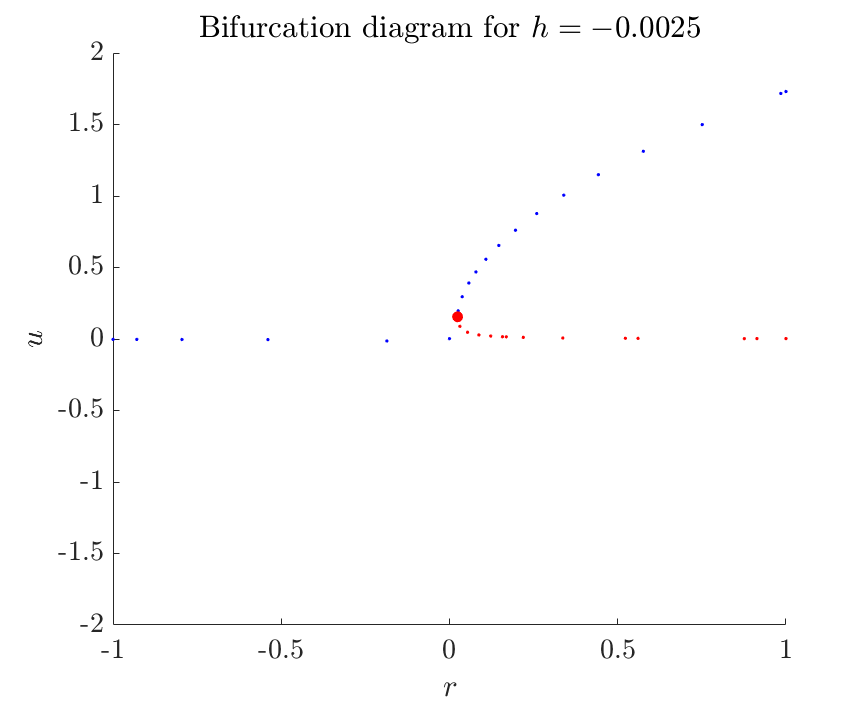
\includegraphics[width=\textwidth]{bs.png}
		\captionsetup{width=0.9\textwidth}
		\caption{Branch switch - step size $\Delta\lambda$ too large (\texttt{h\_max=0.05}).}
		\label{fig:bs}
	\end{subfigure}\hfill

	\begin{subfigure}[b]{0.5\textwidth}
		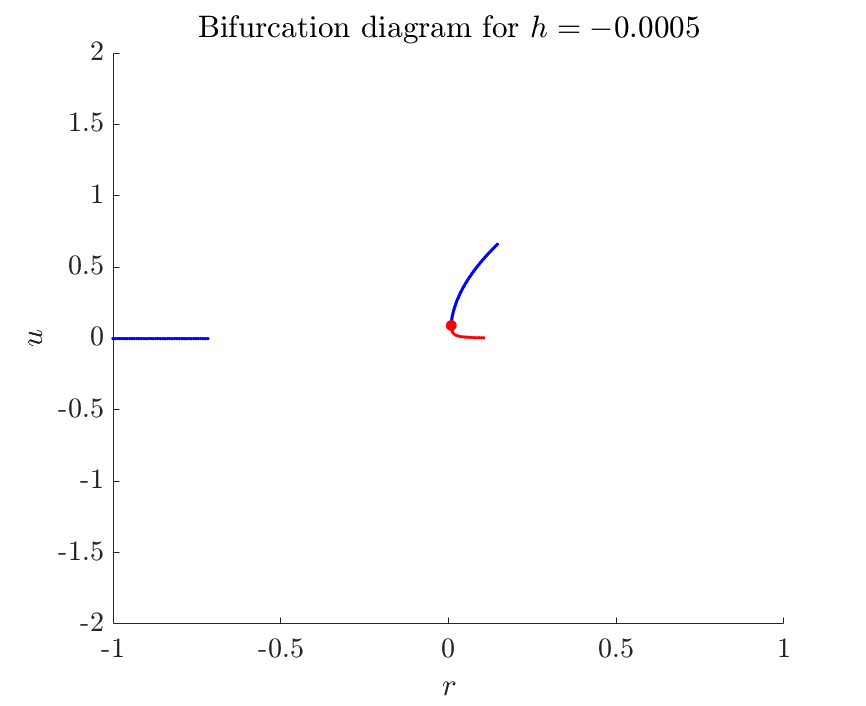
\includegraphics[width=\textwidth]{steps.png}
		\captionsetup{width=0.9\textwidth}
		\caption{Partially computed branches - too few continuation iterations (\texttt{cont - ItMX = 40}).}
		\label{fig:steps}
	\end{subfigure}
	}
	\caption{Bifurcation diagrams in function of $r$ for $h=-0.0005$ and $h=-0.0025$, obtained with \texttt{COCO}.}
\end{figure}
In both plots, the second part of the leftmost branch is lost. This shows why the right continuation parameters are so important.

\newpage
\section{Study of a predator-prey model}
A nonlinear predator-prey model is given, with four physical parameters $a$, $b$, $c$ and $d$. These can have the following interpretations:
\begin{itemize}
	\item $\mathbf{a}$\; This parameter controls the exponential growth of the prey population, or reproduction. This parameter  The value of this parameter is 0.2. 	
 	\item $\mathbf{b}$\; This parameter represents the predator's actions, it is namely the rate of predation. The value of this parameter is 0.5 throughout this assignment.
  	\item $\mathbf{c}$\; The occurrence of natural deaths of the predator population is represented by $c$.
	\item $\mathbf{d}$\; $d$ is an additional parameter which represents emigration of the predators.
\end{itemize}
\subsection{ A qualitative study without external influence}
\paragraph{Question 1}\; When the system is simulated for $x$ in function of time taking $y=0$,
the system always converges to one of three equilibrium points. For this to occur, the initial value
$x_0\in[0,1.5]$. The behaviour of the system in function of the initial condition can be described as such:
\begin{itemize}
	\item $x_0\in[0,0.2)$\; For this initial condition, the equation will always converge to the equilibrium $x^*=0$. This looks
	like a stable equilibrium because of this. However, as the equation is not simulated for $x_0<0$, there can only be stated 
	that $x^*=0$ is at least a half stable equilibrium point, with the stable side in the positive $x-t$-plane.
	\item $x_0\in(0.2,1.5]$\; This range for the initial condition also results in a convergence towards a second stable equilibrium.
	\item $x_0=a=0.2$\; The value of this initial condition is also its respective equilibrium point, $x^*=0.2$. This however, is an 
	unstable equilibrium point, as for any perturbation on the initial condition $x_0=0.2$ 
\end{itemize}
\paragraph{Question 2}\; The steady state solutions with $d=0$ can be computed easily by solving the following system:
\begin{equation*}
	\begin{cases}
		& -x^3 + (1+a)x^2 - ax -bxy=0\\
		& (x-c)y=0
	\end{cases}
\end{equation*}
It can be seen easily that the only two solutions for the second equation are $x^*=c$ and/or $y^*=0$.
These solutions can be filled in in the first equation, yielding the following steady state solutions:

\begin{align}
&x^*=0\;\;\; ,  &y^*=0\label{eq:eq1}\\
&x^*=\frac{a+1+\sqrt{a^2-2a+1}}{2}=a\;\;\; , &y^*=0\label{eq:eq2}\\
&x^*=\frac{a+1-\sqrt{a^2-2a+1}}{2}=1\;\;\; , &y^*=0\label{eq:eq3}\\
&x^*=c\;\;\; , &y^*=\frac{(c-a)(1-c)}{b}\label{eq:eq4}
\end{align}
To determine the stability of these fixed points, the Jacobian needs to be constructed.
Then the determinant and trace can be evaluated to get an idea of the stability.
The Jacobian in symbolic version looks like this:
\begin{equation*}
	\begin{bmatrix}
		-3x^2+2(1+a)-by-a & -bx\\
		y & x-c
	\end{bmatrix}
\end{equation*}
The parameters and variables can then be filled in, and the equilibrium points will be described by means of the parameter $c$.
The results are summarized in \Cref{tb:q2}.
\begin{table}[H]
	\hspace{-10mm}
	\begin{tabular}{c|c|c|c|c|}
	& Equilibrium \eqref{eq:eq1} & Equilibrium \eqref{eq:eq2} & Equilibrium \eqref{eq:eq3} & Equilibrium \eqref{eq:eq4}\\
	\hline
	Determinant ($\Delta$) & $ac$ & $(-a^2+a)(a-c)$ & $(a-1)(1-c)$ & $ c(c - a)(1 - c)$\\
	\hline
	Trace ($\tau$) & $-a-c$ & $-a^2+2a-c$ & $a-c$ & $c(1 + a - 2c)$\\
	\hline
	$\tau^2-4\Delta$ & $(c-a)^2$ & $(c-a^2)^2$ & $\left(c+a-2\right)^2$ & $c(4c^3-4ac^2+(a^2-2a-3)c+4a)$\\\hline
	\end{tabular}
	\captionsetup{width=0.9\textwidth}
	\caption{Trace and determinant of the fixed points with $d=0$.}
	\label{tb:q2}
\end{table}
The stability for these different fixed points can be expressed in function of $c$ with the given values for $a=0.2$ and $b=0.5$.\\
There is an important note to make: linear stability analysis is performed on the Jacobian, which is a good way to get an accurate approximation of the behaviour
of the fixed points. However, when the boundary cases are studied, i.e. the cases when either $\Delta=0$, $\tau=0$ or $\tau^2-4\Delta=0$, this linear \textbf{approximation}
is not reliable as there are still some nonlinear perturbations that are not modeled by the Jacobian. These boundary cases are still included in the analysis below,
but they are just to indicate that they will occur approximately at the values specified (also indicated by ``$\approx$'').
\begin{itemize}
	\item \underline{Equilibrium \eqref{eq:eq1}}: \\ 
		Eigenvalues \& eigenvectors Jacobian: $\lambda_1=-a$ with $v_1=\begin{pmatrix}1\\0\end{pmatrix}$ and\\ $\lambda_2=-c$ with $v_2=\begin{pmatrix}ab/(a - c)\\1\end{pmatrix}$.
		\begin{itemize}
			% \item[\boxed{\textbf{c<0}}  ] Here $\Delta<0$, which means that this will yield a \textbf{saddle point}.
			% From the eigenvalues and eigenvectors the stable and unstable manifold can be derived. The stable manifold is spanned by $v_1$ as $\lambda_1<0$ and the unstable manifold is spanned by
			% $v_2$ as $\lambda_2$ is positive.
   			\item[\boxed{\mathbf{c\approx0}}  ] $\Delta=0$, which means that there is a \textbf{line of (stable) fixed points} present as one of the eigenvalues becomes 0.
      		\item[\boxed{\textbf{c>0}}  ] $\Delta>0$, $\tau<0$. $\tau^2-4\Delta>0$ except for when $\mathbf{c\approx a}$, when $\tau^2-4\Delta$ will become 0. When 
			  $c\approx a$, a \textbf{stable degenerate node} will arise.\\ The other values for $c>0$ will yield a \textbf{stable node}.
			  To get its slowest eigendirection, the eigenvector corresponding to the eigenvalue that is smallest in absolute value needs to be found.
			  The slowest eigendirection will depend on if $a<c$ or not.
			  If $a<c$, $v_1$ is the slowest eigendirection, and if $a>c$, $v_2$ is the slowest eigendirection of the stable node.
		\end{itemize}
	\item \underline{Equilibrium \eqref{eq:eq2}}: \\
		Eigenvalues \& eigenvectors Jacobian: $\lambda_1=-a^2+a$ with $v_1=\begin{pmatrix}1\\0\end{pmatrix}$ and\\ $\lambda_2=a-c$ with $v_2=\begin{pmatrix}0\\- a^2 + a\end{pmatrix}$.
		\begin{itemize}
			\item[\boxed{\textbf{0<c<a}}  ] $\Delta>0$ and $\tau>0$, as well as $\tau^2-4\Delta>0$. This means that this fixed point will be an \textbf{unstable node}.\\
			The slowest eigendirection again depends on $c$: if $c<a^2$, then it is $v_1$ as $\lambda_1$ is the smallest
			eigenvalue. If $a^2<c<a$, then $v_2$ is the slowest eigendirection.\\
			A special case occurs when $c\approx a^2$. Then $\tau^2-4\Delta=0$, so this fixed point will become an unstable degenerate node.
			\item[\boxed{\mathbf{c\approx a}}  ] $\Delta=0$, so one of the eigenvalues is zero ($\lambda_2=0$). There will be a whole \textbf{line of unstable fixed points}, as $\lambda_1>0$.
   			\item[\boxed{\textbf{c>a}}  ] $\Delta<0$, so this fixed point will become a \textbf{saddle node}. The unstable manifold is spanned by $v_1$ ($\lambda_1>0$) and the stable 
			   manifold by $v_2$ ($\lambda_2<0$).
		\end{itemize}
	\item \underline{Equilibrium \eqref{eq:eq3}}: \\
		Eigenvalues \& eigenvectors Jacobian: $\lambda_1=a-1$ with $v_1=\begin{pmatrix}1\\0\end{pmatrix}$ and\\ $\lambda_2=1-c$ with $v_2=\begin{pmatrix}b/(c + a - 2)\\1\end{pmatrix}$.
		\begin{itemize}
			\item[\boxed{\textbf{0<c<1}}  ] $\Delta<0$, so a \textbf{saddle node} is present. The stable manifold is spanned by $v_1$ as $\lambda_1<0$ and the unstable manifold is defined
			by $v_2$ as $\lambda_2>0$ in this case.
   			\item[\boxed{\mathbf{c\approx 1}}  ] $\Delta=0$, a \textbf{line of (stable) fixed points} is present.
      		\item[\boxed{\textbf{c>1}}  ] $\Delta>0$, $\tau<0$. $\tau^2-4\Delta$ can vary, when it occurs that $c\approx 3-0.75a=1.5$, then $\tau^2-4\Delta=0$ and a 
			  \textbf{degenerate node} will arise. \\ When $c<3-0.75a=1.5$, then $\tau^2-4\Delta>0$ and this point will become a \textbf{stable node}. The slow eigendirection again depends on $c$:
			  when $1<c<1.5<2-a$, $\lambda_2$ will be the smallest eigenvalue (in absolute value) and $v_2$ will define the slowest eigendirection.\\
			%   A special case occurs when $c\approx 2-a$, which causes that $\tau^2-4\Delta=0$, so a stable degenerate node arises.
		\end{itemize}
	\item \underline{Equilibrium \eqref{eq:eq4}}: \\
		\begin{itemize}
			% \item[\boxed{\textbf{c<0}}  ] $\Delta>0$ and $\tau<0$. Regarding $\tau^2-4\Delta$, there are different possibilities. When $a=0.2$ is filled in, $\tau^2-4\Delta=0$ for 
			% for a value $c\approx-0.9318$; a \textbf{stable degenerate node} is established.\\ When $c<-0.9318$, $\tau^2-4\Delta>0$, so a \textbf{stable node} arises.\\ When $c>-0.9318$, 
			% $\tau^2-4\Delta<0$, so a \textbf{stable spiral} occurs.
			\item[\boxed{\mathbf{c\approx0}}  ] $\Delta=\tau=0$. A \textbf{plane of neutrally stable fixed points} is present as both eigenvalues of the Jacobian are zero.
   			\item[\boxed{\textbf{0<c<a}\; \& \;\textbf{c>1}}  ] $\Delta<0$, so then this fixed point becomes a \textbf{saddle node}.
      		\item[\boxed{\textbf{a<c<1}}  ] $\Delta>0$: \begin{itemize}[leftmargin=20mm]
															\item[\underline{a < c < 0.241}] $\tau>0$ and $\tau^2-4\Delta>0$ $\Rightarrow$ \textbf{unstable node}\\
															When $c\approx0.241$, $\tau^2-4\Delta=0$ $\Rightarrow$ \textbf{(unstable) degenerate node}
               												\item[\underline{0.241 < c < (1+a)/2}] $\tau>0$ and $\tau^2-4\Delta<0$ $\Rightarrow$ \textbf{unstable spiral}\\
															   When $c\approx(1+a/2)$, $\tau=0$ $\Rightarrow$ \textbf{neutrally stable center}.
															\item[\underline{(1+a)/2 < c < 0.89}] $\tau<0$ and $\tau^2-4\Delta<0$ $\Rightarrow$ \textbf{stable spiral}\\
															When $c\approx0.89$, $\tau^2-4\Delta=0$ $\Rightarrow$ \textbf{(stable) degenerate node}
															\item[\underline{0.89 < c < 1}] $\tau<0$ and $\tau^2-4\Delta>0$ $\Rightarrow$ \textbf{stable node}\\
														\end{itemize}
   			\item[\boxed{\mathbf{c\approx 1}}  ] $\Delta=0$, so a whole \textbf{line of (stable) nodes} is present.\\
		\end{itemize}
\end{itemize}
An example of each parameter region listed here is shown \Cref{fig:stab2}. The boundary cases are not added, as the values that are computed analytically 
for the linear approximation of the system don't always correspond to the real nonlinear system.\\
To summarize, the characteristics of the phase portrait change at values $c\approx0$, $c\approx a$, $c\approx0.241$, $c\approx(1+a)/2$, $c\approx0.89$ and $c \approx1$.

\paragraph{Question 3}\; When plotting the phase portrait using \texttt{PPLANE}, the plots correspond to the analytical results.\\
There can be seen that the stable manifolds of the saddle nodes often serve as separatrices that divide the phase diagram in two separate basins
of attraction, where the trajectories of the simulations get repulsed into different stable fixed points.\\
Unstable manifolds also serves as a boundary between two types of trajectories. Namely, trajectories that come from opposite sides of the unstable manifold, come from different
``basins of repulsion'' and come together on the unstable manifold.\\
The separatrices can be found by using a simulation in \texttt{PPLANE} and looking at their behaviour and location. Then an analytical technique can be applied to find the 
exact eigendirections of the saddle node. In \Cref{fig:ph3} the basins of attraction are indicated.

\paragraph{Question 4}\; Using the results from the previous questions, a qualitative overview of the phase diagram in function of c can be given.
This is done by means of \Cref{tb:pd4}, where the most important observations are summarized. For an explanation in more detail, I refer to Question 3.
Plots of the respective states of the system are shown in \Cref{fig:stab2}.
The boundary cases are not treated here, as the analytical linear approximation doesn't fully correspond to the nonlinear behaviour.
\begin{table}[H]
	\begin{tabular}{|c|c|c|c|c|}\hline
	& Equilibrium \eqref{eq:eq1} & Equilibrium \eqref{eq:eq2} & Equilibrium \eqref{eq:eq3} & Equilibrium \eqref{eq:eq4}\\
	\hline
	$0<c<a$ & Stable node & Unstable node & Saddle node & Saddle node\\\hline
	$a < c < 0.241$ & Stable node & Saddle node & Saddle node & Unstable node\\\hline
	$0.241 < c < (1+a)/2$ & Stable node & Saddle node & Saddle node & Unstable spiral\\\hline
	$(1+a)/2 < c < 0.89$ & Stable node & Saddle node & Saddle node & Stable spiral\\\hline
	$0.89 < c < 1$ & Stable node & Saddle node & Saddle node & Stable node\\\hline
	$c>1$ & Stable node & Saddle node & Stable node & Saddle node \\\hline
	\end{tabular}
	\captionsetup{width=0.9\textwidth}
	\caption{Evolution of the equilibrium points in function of $c$.}
	\label{tb:pd4}
\end{table}
For \Cref{eq:eq4}, the evolution of the eigenvalues of the Jacobian in function of $c$ in the complex plane can be seen in \Cref*{fig:ev4}, two plots for 
both the real and imaginary part. There can be seen that a pair of real eigenvalues transition into a pair of complex conjugate eigenvalues at $c\approx0.241$.
Later they transition back into a pair of real eigenvalues at $c\approx 0.89$. In the phase plane these transitions correspond to going from a node to a spiral, 
and then back to a node.\\
When looking at the real part, there can be seen that sometimes one or both eigenvalues change sign, which has a change of stability characteristics as a consequence.
Looking at the nodes, the real part simply decides the stability of them. In this case a saddle node is present for $0<c<a=0.2$ and $c<1$, an unstable node for 
$a<c<0.241$ and a stable node for $0.89<c<1$. In between one of the eigenvalues is zero and a degenerate node is present.\\
For the spirals, the real part of both eigenvalues switches sign at $c\approx(1+a)/2=0.6$, and like this a stable spiral ($0.241<c<0.6$) transitions into an 
unstable spiral ($0.6<c<0.89$). 
This indicates that a Hopf bifurcation is present at $c\approx0.6$. To decide whether it is a super- or subcritical one, 
the numerical phase portrait was inspected. From there the behaviour of a supercritical Hopf bifurcation can be deducted, see also \Cref{fig:bf4}.

\paragraph{Question 5}\; The interval $[c_1,c_2]$ that was given to me is $[0.51,0.61]$. The global bifurcation that is in play here looks like a homoclinic bifurcation,
but this time interacting with two saddle nodes instead of one, so it could be called a heteroclinic bifurcation.
at $c\approx0.54$. For $0.51<c<0.54$, there is no limit cycle present, just an unstable orbit at \Cref{eq:eq4}. For values $0.54<c<0.61$ there arises a limit cycle at \Cref{eq:eq4}
that is trapped between the two stable manifolds of saddle nodes \Cref{eq:eq2} and \Cref{eq:eq3}. The larger $c$ gets, the smaller the orbit, till it completely disappears
at $c\approx(1+a)/2=0.6$ and a stable spiral arises, i.e. the Hopf bifurcation mentioned in Question 4.
The bifurcation can be verified by using the scaling law for the period of the limit cycle. This period $T$ can be approximated by numerically solving the system
sufficiently far in time for $x$ and $y$ and observing the periods that arise for $0.54<c<0.61$. A clear logarithmic behaviour is seen when $c$ is increased above 0.54 which
corresponds to the scaling law of the period of the cycle for a homoclinic bifurcation (ln($\mu$)). This is shown in \Cref{fig:T5} where the period of the limit cycle (which
is the same as the one for $x(t)+y(t)$) is monitored in function of $c$.
Also, for values of $c_{crit}$ around the bifuration, the period becomes infinite because the trajectories get stuck in the heteroclinic orbit, which removes the periodicity.
A figure for the critical value $c_{crit}=0.54$ is shown in \Cref{fig:homcl5}.

\paragraph{Question 6}\; The evolution of the solutions for two different limit cycles is studied. For this, the equilibrium point that was studied in Question 4 can be used.
\begin{itemize}
	\item[\textbf{i.}] When $c\approx0.54$, a limit cycle close to a heteroclinic cycle is present. There can be seen that both $x$ and $y$
	(but in particular $y$) have peaked oscillations with a sharp maximum but a smoother minimum. These peaks most likely occur by the saddle points it interacts with,
	as the limit cycle becomes a more discontinuous there. Both oscillations look quite different, both in shape and in amplitude, this is because of the 
	irregular shape of the limit cycle. 
	\item[\textbf{ii.}] For values of $c\approx0.6$, the limit cycle becomes a lot smaller and almost disappears, but the shape of it comes close to a regular circle,
	which indicates a harmonic oscillation. Indeed, when looking at the solutions, a sinusoidal behaviour can be noticed in both solutions, which points to a harmonic 
	oscillation. Both $x$ and $y$ look very similar, both in shape and in amplitude. Only a phase shift between the two is present.
\end{itemize}
Simulations of both cases have been performed and their solutions are depicted in \Cref{fig:cycl6}.
\subsection{Bifurcation analysis}
\paragraph{Question 1}\; The bifurcation diagram for $d=0$ in the $(c,x)$-plane is drawn in \Cref{fig:bifd0}. Green represents the saddle nodes, red the unstable nodes/spirals and
blue the stable nodes/spirals. The four equilibrium points can be distinguished easily. Three of the equilibria are horizontal lines, as their location doesn't change, 
namely Equilibrium \eqref{eq:eq1}, \eqref{eq:eq2} and \eqref{eq:eq3}. Equilibrium \eqref{eq:eq4} has $x^*=c$, so a line with slope 1 is present, and sometimes interacts with 
the horizontal lines.
There can be seen that two bifurcation points are present,
both of which represent transcritical bifurcations: 
\begin{itemize}
	\item $\mathbf{c\approx a=0.2}$: This is the point where Equilibrium \eqref{eq:eq2} transitions from an unstable node to a saddle node, and where \eqref{eq:eq4} becomes
	an unstable node, coming from a saddle node. 
	\item $\mathbf{c\approx 1}$: Here Equilibrium \eqref{eq:eq4} transitions from a stable node back to a saddle node. Equilibrium \eqref{eq:eq3} goes from a saddle node to 
	stable node.
\end{itemize}
Equilibrium \eqref{eq:eq1} stays a stable node throughout, as seen before. At $c\approx (1+a)/2$, the stability of Equilibrium \eqref{eq:eq4} changes, as it goes from an 
unstable spiral to a stable one, as also seen in the previous analysis.\\
The plot for the $(c,y)$-plane is also included in \Cref{fig:bifd0} because it is useful for the next question, and the interval $[-0.5,0.1]$ of $c$ is purely illustrative. 

\paragraph{Question 2}\; When $d$ is taken different from zero, the bifurcation diagram changes and the transcritical bifurcations split into saddle node bifurcations.
The intervals where $c\in[-0.5, 0.1]$ are meant as an illustration for what the branches look like further down the road.\\
\begin{itemize}
	\item[\boxed{\mathbf{d=0.01}}  ] The plot of the bifurcation diagram in the $(c,x)$- and $(c,y)$-plane is depicted in \Cref{fig:bifd+}.
	\begin{itemize}
		\item $\mathbf{(c,x)\text{-plane}}$:  Here can be seen that both transcritical bifurcations disappear compared to $d=0$. The one at $c\approx1$ splits up into two saddle node 
		bifurcations, while the branches bifurcation at $c\approx a$ move away from each other so that the bifuration point vanishes.
		\item $\mathbf{(c,y)\text{-plane}}$:  The same thing happens in the $(c,y)$ projection. The branches are located differently and have a different shape.
		When $d=0$, the first three equilibria all overlap as they all habe $y^*=0$. Equilibrium \eqref{eq:eq4} is quadratic in $c$ so this forms a parabola which intersects the
		$y=0$-line, causing transcritical bifurcations as well.\\
		For $d=0.01$, the bifuration point at $c\approx1$ again splits up into two turning points and at $c\approx a$ the bifurcation disappears.
	\end{itemize}
	\item[\boxed{\mathbf{d=-0.01}}  ] The bifurcation diagrams are shown in \Cref{fig:bifd-}
\end{itemize}


\end{document}